\section{Experiments}
\label{sec:experiments}




\subsection{Sketch Interface}
We develop a sketch-based interface which allows common users to describe their desired face and part shapes by a few strokes. Once the user finishes his drawing, the generated face image is shown on the right \td{bottom of the sketch? This will be helpful for local editing.}, as Fig.~\ref{fig:interface} shows.
The user is allowed to edit the sketch by erasing strokes or adding new stroke to change eye shapes, noses shapes, eyebrows, and so on.
%
Each round of face image generation after users' modification takes about \td{... seconds on a XXX GPU with xxGB memory.}
%




\begin{figure}
	\centering
	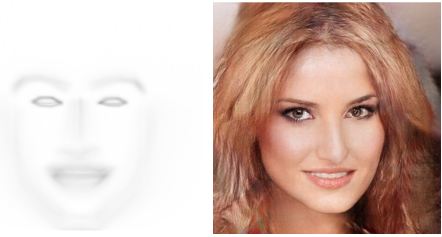
\includegraphics[width=\columnwidth]{figs/interface.png}
	\caption{Sketch interface. \td{Full interface with editing tools.}}
	\label{fig:interface}
\end{figure}
 


\subsection{Comparison with Image Translation networks}

Existing DNNs for image translation can be trained for sketch-photo translation using the paired dataset.

\subsection{Comparison with Image Editing}


\subsection{Limitations and future work}

\td{Add color}

\td{Combine with attribute}